\section{Material and Method}

\subsection{Implementation of the Workflow and Interpretation of the Results}

The protocol used in this study can be splited in 3 steps described here.
The datasets used, \acrfull{de} and Pathway Enrichment analysis are then described in more details in the next sections.
\begin{enumerate}
    \item \textbf{Define a list of genes of interest} : In this step we use RNA-Seq data to look for the genes that are deregulated in glioblastoma. 
    We compared, gene expression between samples taken from patien's tumour with healthy astrocytes cells.
    \item \textbf{Find the deregulated pathways} : We use the list of deregulated genes found in the previous step as input to pathway enrichment.
    Pathway enrichment analysis search for pathways that are enriched in the list of genes.
    As a result, pathway enrichment analysis look for the pathways that altered in glioblastoma when using a list of deregulated genes in this disease.
    We selected two methods G:Profiler and \acrfull{gsea}, and two databases \acrfull{kegg} and Reactome.
    \item \textbf{Interpret the results} : We compared the differences in categories enriched between the tools for each databases.
    As both \acrshort{kegg} and Reactome organize their pathways in a hierarchical manner we can map each pathways to their \textit{Top Level Pathway}, the highest pathway in the tree.
    Those \textit{Top Level Pathway} are too general to bring deep insight into biological processes affected, yet we used them to define biological categories (For example Cell-Cyle).
    Therefore, we defined biological categories for the two database and mapped each of the pathways to one of those categories.
    hierarchical ordering of the pathways was retrieved by interrogating the web API of both databases.
    To avoid false positive and reduce the number of pathways found, we then selected only the pathways that are below the significant threshold in both G:Profiler and \acrshort{gsea}.
\end{enumerate}
All the data analysis were carried out with the R programming langage.
To perform G:Profiler pathway enrichment we used the official R librarie (version \textbf{0.2.1}).
Although an R script is available on the \acrshort{gsea} webpage, it is not maintained by the team.
Instead we used the \textit{fgsea} package for Fast Gene Set Enrichment Analysis available on Bioconductor (version \textbf{1.12.0}) \cite*{Korotkevich2021}.
We used ggplot2 (version \textbf{3.3.6}) and rmarkdown (version \textbf{2.14}) to generate the plots in this publication and the report (in supplementary materials).

\begin{figure}
    \centering
    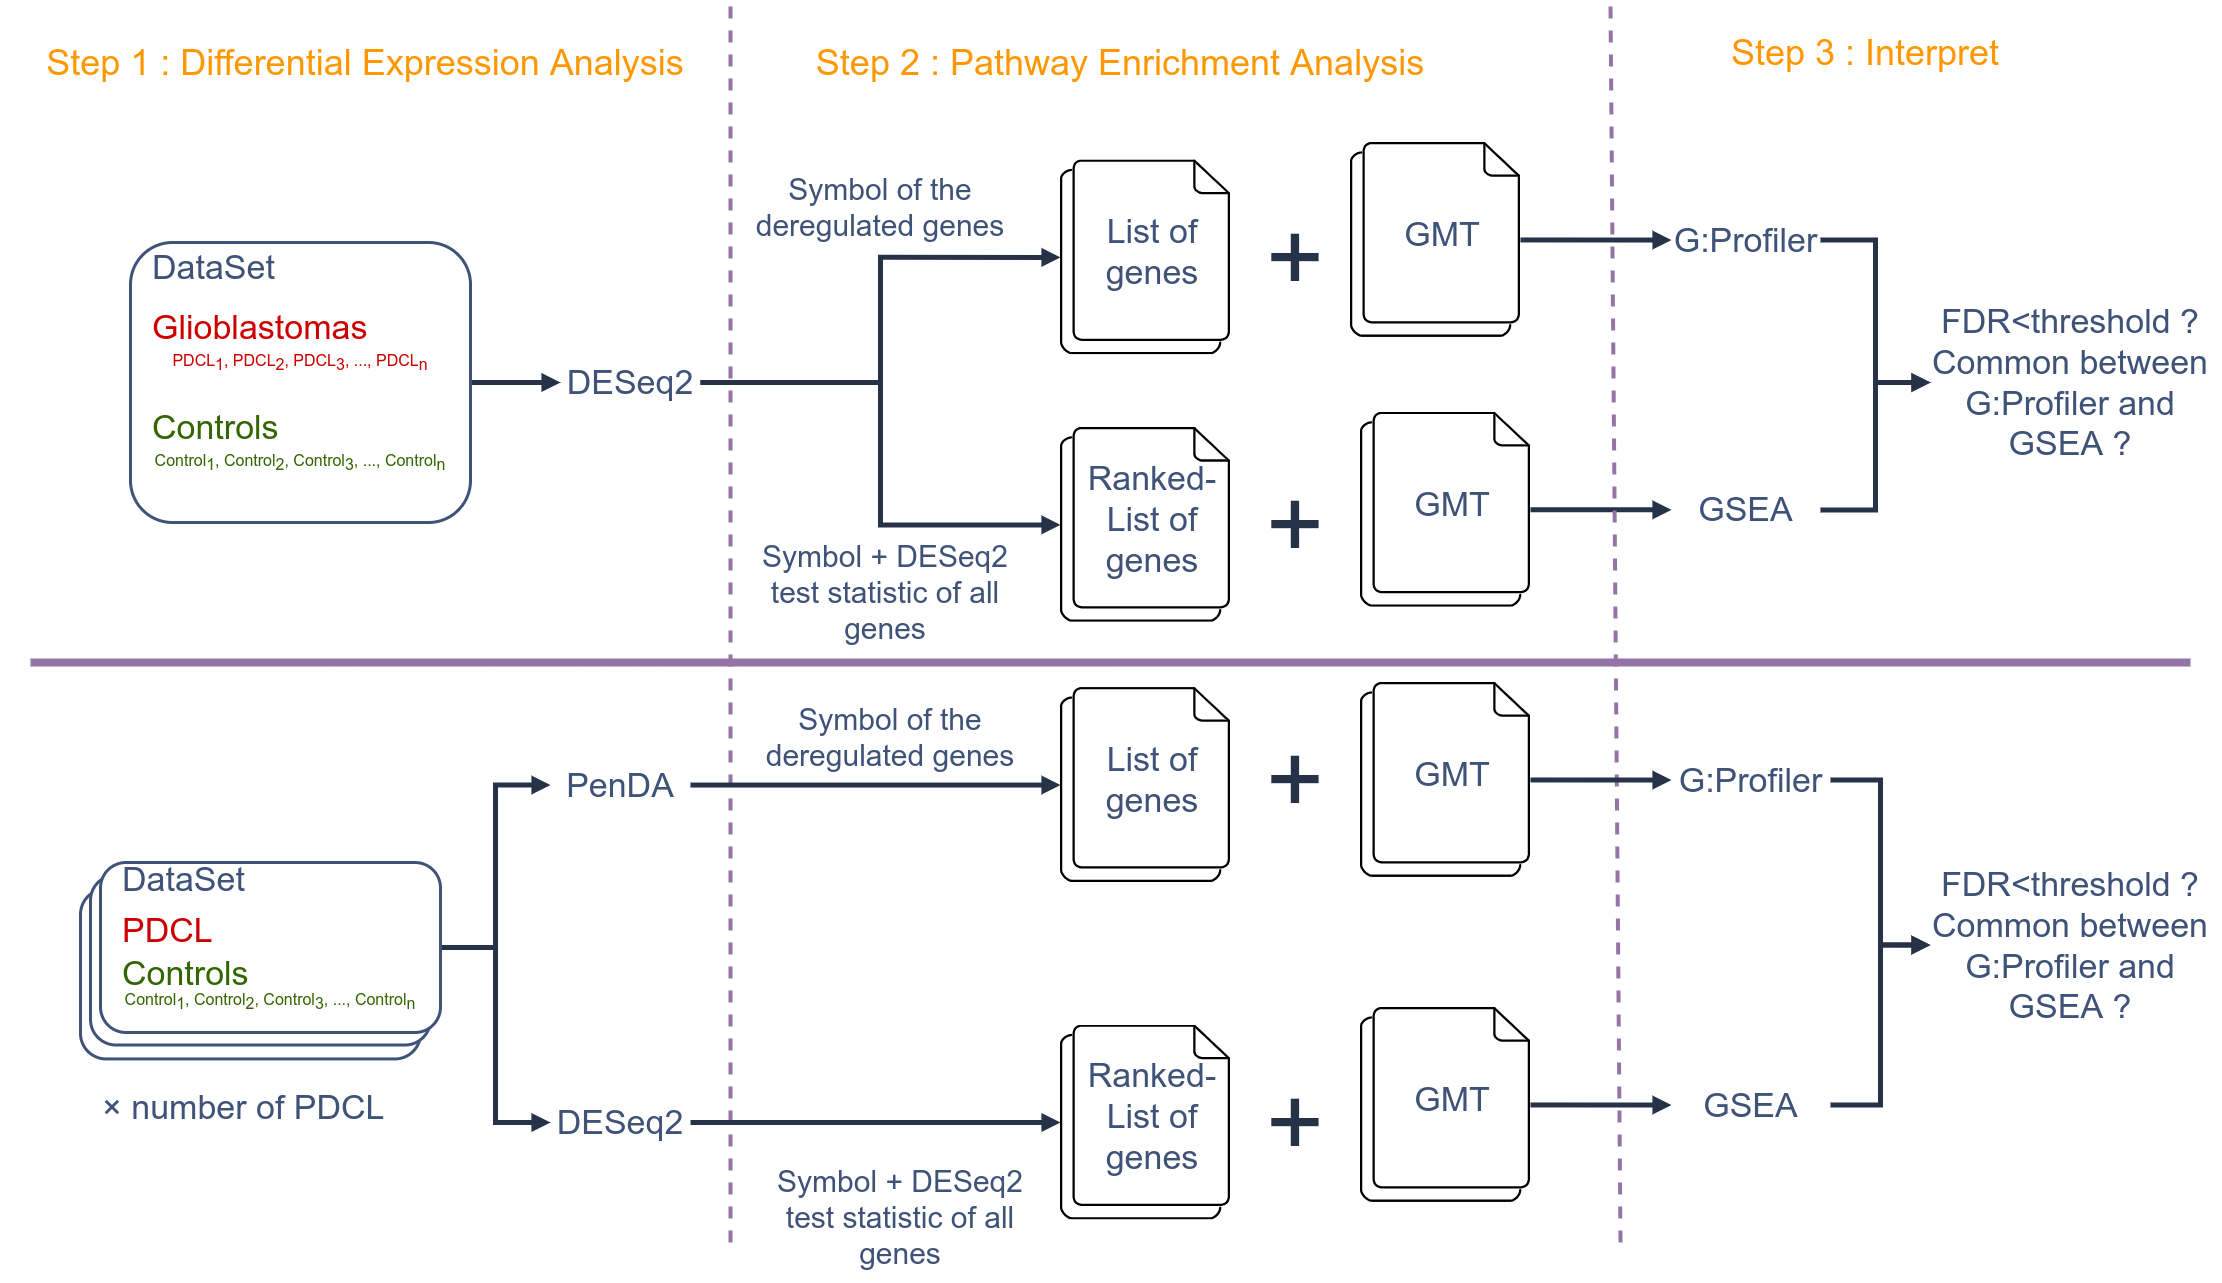
\includegraphics[width=\textwidth]{img/workflow-diagram.png}
    \caption{
        Diagram of the overall approach used in this paper.
    }
    \label{fig:workflow-diagram}
\end{figure}

\subsection{Data Sets}

Cells were taken from tumor of 20 patients diagnosed with glioblastoma, they were  then cultured \textit{in vitro}.
RNA-Seq analysis was then conducted to obtain the raw counts of approximately 20,000 genes for each samples.
Due to licensing limitations, data cannot be shared with the publication and all biological experiments were conducted by the \acrfull{icm} in Paris.
\todo{check the origin of the pdcl dataset}
We will refer to this dataset as \acrfull{pdcl}.
Only one replicate per sample is available.

Because the \acrshort{pdcl} dataset does not includes matching control samples, we compared them to astrocytes RNA-Seq data from a study on the characterization of different astrocytic models by Lundin  al \cite*{Lundin2018}.
Raw counts data are available for download on the \acrfull{geo} platform under the accession number \textbf{GSE109001}.
The dataset contain 4 samples of different astrocyte cell lines with 3 replicates per samples.
The accession number and the name of the samples are listed in table \ref*{table:list-control-samples}.
At the time of the publication, data were last updated on January 29, 2019.

\begin{table}
    \centering
    \begin{tabular}{ |c|c| }
        \hline
        Accession Number & Sample name \\
        \hline
        GSM2927872 & AF22\_NES-Astro\_d29\_Br1 \\
        GSM2927873 & AF22\_NES-Astro\_d29\_Br2 \\
        GSM2927874 & AF22\_NES-Astro\_d29\_Br3 \\
        \hline
        GSM2927881 & iCellAstro\_Br1 \\
        GSM2927882 & iCellAstro\_Br2 \\
        GSM2927883 & iCellAstro\_Br3 \\
        \hline
        GSM2927884 & CCF\_Br1 \\
        GSM2927885 & CCF\_Br2 \\
        GSM2927886 & CCF\_Br3 \\
        \hline
        GSM2927887 & phaAstro\_Br1 \\ 
        GSM2927888 & phaAstro\_Br2 \\ 
        GSM2927889 & phaAstro\_Br3 \\ 
        \hline
    \end{tabular}
    \caption{
        List of samples with their accession number used as the control condition.
        Each samples can be either downloaded separately or as one raw count file in text format using the accession number \textbf{GSE109001} on \acrshort{geo}.
    }
    \label{table:list-control-samples}
\end{table}

We also compare the pathways altered in the \acrshort{pdcl} dataset with the pathways found altered in a dataset accessible on \acrshort{tcga} database. 
We downloaded glioblastoma gene expression data from the TCGA-GBM project for both tumour and control samples.
The lastest \acrshort{tcga} version available \textbf{v33.1} was released on May 31 2022, transcriptomes profilling for all \acrshort{tcga} projects were updated in version \textbf{v32.0} released March 29 2022.
\todo{redo analysis with updated database}
RNA quantification was performed on primary or recurrent tumour for the glioblastoma samples, and on solid tissue for control samples.
Importantly, very few normal transcriptomes profilling are available for control samples in the TCGA-GBM project and none are available for TCGA-LGG (Lower Grade Glioma data).
Thus, this dataset will be over-represented by tumourous samples with 169 tumour samples and 5 control samples.

\subsection{Differential Expression Analysis}

Before we assess the pathways that are altered in case of glioblastoma we need to look for genes whose expression are deregulated.
A \acrfull{de} analysis consist of comparing the expression of a gene, the quantity of RNA produced by a gene, between two conditions (usually disease versus a control).
Results generated during this step are then used as input to perform Pathway Enrichment analysis to associate the list of deregulated genes with a list of biological pathways.
To quantify the expression of a gene, reads produced during an RNA-Seq experiment are mapped to the genes of a reference genome.
The number of mapped reads is computed for each genes giving a raw value called raw counts.
Factors such as transcript length, total number of reads and sequencing biases can impact the raw counts value. 
Therefore, raw counts need to be normalized to obtain a value suitable for comparison \cite*{Conesa2016}.
Different tools are available to perform \acrshort{de} analysis such as edgeR \cite*{Robinson2010}, Limma \cite*{Ritchie2015}, DESeq2 \cite*{Love2014} and \acrshort{penda} \cite*{Richard2020}.
In this study, we selected DESeq2 \cite*{Love2014} and \acrfull{penda} to carry out the \acrshort{de} analysis.

\acrshort{de} analysis was performed on the two datasets \acrshort{pdcl} and \acrshort{tcga} where we compared all the tumourous samples against all the normal samples (glioblastoma versus normal).
With this approach, we identify a typical glioblastoma profile or the typical gene deregulations in the case of glioblastoma that is used in the pathway enrichment analysis.
Glioblastoma are known to be heterogeneous tumours, hindering therapeutic success \cite*{Neftel2019,Delgado-Lopez2016, Quinones2018}.
Since the approach described does not account for heterogeneity between patients, we compared each samples from the \acrshort{pdcl} dataset one by one with all the controls.
In this second approach, we define the deregulated pathways for each samples to determine which pathways are the most, or the least, commonly deregulated in our dataset.
However, the \acrshort{pdcl} dataset contain one replicate per patient while the hypothesis used for statistical testing in DESeq2 assume several replicates.
This lead to reduced accuracy and reliability of the results of DESeq2 as the conditions to use this tool are not met anymore.
In this regard, we used the results generated with \acrshort{penda} on each samples of \acrshort{pdcl} dataset during a previous study carried out in our team.
Results from DESeq2 and \acrshort{penda} generated during this step are then used for pathway enrichment to determine the biological pathways affected.

DESeq2 uses a negative bionomial distribution (also called gamma-Poisson distribution) to model read counts and perform a Wald-Test to test for differential expression.
As DESeq2 includes a built-in normalization method, only raw counts can be used as input to the tool.
It also perform an automated detection of outliers, detection of gene with low counts, estimation of model factors and gene expression dispersion.
The $log_2$ fold change value is a numeric value used to quantify the strength and direction of deregulation (up or down) between a condition and the control.
We selected DESeq2 for the features cited above, its ease of use and its overall performance \cite*{Love2014}.

\acrshort{penda} is a rank-based method to perform \acrshort{de} using a sample from the condition to test for differential expression and a reference dataset \cite*{Richard2020}.
In comparison, population scale analysis tools like DESeq2 usually model the data using a distribution law and perform a statistical test to detect differential expression.
Those methods were designed to investigate typical gene deregulations patterns, consequently they do not provide informations at the individual scale.
They are also sensitive to batch effets and the choice of normalization applied.
With all this limitations in mind, \acrshort{penda} was designed to investigate gene expression data at the individual scale with robustness to batch and normalization effects.

\subsection{Pathway Enrichment Analysis}

Here, we used the results of the \acrlong{de} analysis described above as input to investigate the deregulated pathways in the \acrshort{pdcl} and \acrshort{tcga}.
The \acrlong{pdcl} dataset was analyzed at both the population and the patient scale while the \acrshort{tcga} was only examined at the population scale.
Here we selected the two tools G:Profiler and \acrfull{gsea} to run the pathway enrichment analysis.

G:Profiler is a tool for finding biological processes enriched in a list of genes (for example a list of deregulated genes or a list of mutated genes) accessible either online using their web interface or using their API and libraries \cite*{Raudvere2019}.
It search for pathways or biological categories which are over-represented in a list of genes using the cumulative hypergeometric test.
g:SCS, a new method for multiple testing correction developped by the G:Profiler team, is implemented ad used by default.
Users are able to choose the more known Bonferroni and \acrshort{fdr} correction method.

\acrfull{gsea} is a rank-based method developped by Subramanian \textit{et al} to interpret gene expression data with a java application available for download.
Genes in the list feed to the tools must be ordered using a ranking metric that can be either a positive or negative value.
For example, the user can order the genes using the difference in expression between two conditions (fold change).
The \acrshort{gsea} approach determine whether the genes involved into a gene set are mostly distributed at the top or the bottom of the gene list.
An \acrfull{es} is computed for each gene set by running through the list of genes, increasing a running-sum statistic by the rank of the gene if the gene is present in the current gene set or decreasing the statistic otherwise.
The maximum deviation from zero computed during the run is the \acrshort{es}, it correpond to a weighted Kolmogorov-Smirnov-like statistic.
Then a null distribution for the \acrshort{es} is computed by permutating the gene in the dataset (phenotype permutation is also available) to estimate the significance of the observed \acrshort{es}.
\acrshort{gsea} use the \acrshort{fdr} method to adjust for multiple hypothesis testing.

biological informaton must be provided to pathway enrichment tools as gene set, a group of genes sharing a common biological feature (for example a biological function or chromosomal location).
Both G:Profiler and \acrshort{gsea} need biological information in a tabular format called \acrfull{gmt} where each rows is a gene set, in this study gene sets are pathways.
The first column of the file contain the pathway ID, the second column contain a description and the remaining column are all the genes involved in the pathway.
G:Profiler is updated regularly with the most common databases such as \acrshort{kegg}, Reactome, WikiPathways, miRTarBase and Gene Ontology.
All gene set can be downloaded from the G:Profiler website, except for \acrshort{kegg} and TRANSFACT due to data licensing limitations.
\acrshort{gsea} include built-in gene set from the Molecular Singatures Database (MSigDB), they also can be downloaded.
G:Profiler and \acrshort{gsea} allow the user to submit custom \acrshort{gmt} file as well.

Despite both of them need a list of genes, G:Profiler need only the genes symbol as input while for \acrshort{gsea}, each genes must be assigned a metric value.
A study from Zyla \textit{et al} has shown that the \acrshort{gsea} metric used can impact the results \cite*{Zyla2017}.
They evaluated the performance of 16 differents metrics and found that the absolute value of the Moderated Welch Test statistic, the Minimum Significant Difference, the absolute value of the Signal to Noise ratio and the Baumgartner-Weiss-Schindler test statistic give the best outcome.
Among the best performing metrics cited, some are computed as part of a statistical test.
Thus, we ranked the genes of the dataset with the statistic of the Wald-Test computed by DESeq2 before we run \acrshort{gsea}.
The Wald-Test statistic has 2 features usefull for ranking the genes : (1) the statistic value has the same sign as the $log_2$ Fold Change, giving the direction of deregulation (up or down) and providing biological information; (2) the higher the absolute value of the statistic is, the more significant the difference between the condition tested and the control is.
Therefore, the Wald-Test statistic combine both biological and statistical informations, suggesting it is a valuable metric for running \acrshort{gsea} analysis.
To reduce the number of pathways to investigate in the litterature and to ensure the reliability of the result, we will select the pathways that are found deregulated both by G:Profiler and \acrshort{gsea}.
We consider a pathway deregulated if the adjusted p-value is below $0.1$.
To be consistent between G:Profiler and \acrshort{gsea}, we choose the \acrfull{fdr} correction method for multiple hypothesis testing.
We downloaded gene set from \acrshort{kegg} \cite*{Kanehisa2019} and Reactome \cite*{Gillespie2022}, two biological databases with curated set of data.
A same pathway can have a different definition between databases, the glycolysis is defined as \textit{canonical glycolysis} in Gene Ontology, \textit{glycolysis} in Reactome and \textit{Glycolysis/Gluconeogenesis} in \acrshort{kegg}.
As the genes included in each pathways may change following the database, comparing the results obtained with different sources would reveal pathways that may not appear with one database.
It is beneficial to exclude small and large pathways as : (1) small pathways are redundant with larger pathways while large pathways are often too general (metabolism, cell-cycle); (2) small pathways are never picked up by pathway enrichment tools while large pathway tend to always show up in the results; (3) higher number of pathways in the data makes multiple-testing correction more strict \cite*{Reimand2019}.
Pathways size of 10-15 to 200-500 genes are recommanded yet sizes of 2,000 genes can be found in the litterature \cite*{Reimand2019}.
In this paper, we kept pathways of 15 to 1,000 genes.
After validation of the pathways found by the enrichment tools, we filtered out pathways associated to the \textit{Disease} categorie as they do not bring usefull information (example : \textit{Glioma} from \acrshort{kegg}).
